\section{Yield Curve Forecasting}
    \subsection{Stationarity and cointegration research of the bond yields}
        Stationarity and absence of cointegration are the key assumption for the correctness of many models.
        We shall test the stationarity of the bond yields and the cointegration of the yield curve and the macroeconomic variables.
        \subsubsection{Stationarity}
            In order to test the stationarity of the bond yields, we shall use the \emph{Augmented Dickey-Fuller test} (ADF test).
            The null hypothesis of the test is that the time series is non-stationary.
            The ADF test is a unit root test, which means that it determines how strongly a time series is defined by a trend.
            The test is based on the assumption that the time series is a random walk with drift.
            The test is performed using the \texttt{ur.df} function from the \texttt{urca} package in R.
            The results of the test are presented in Table \ref{tab:adftestForYields} (yields) and Table 
            \ref{tab:adftestForYieldsDifference} (first difference).
            \subimport{results/BondDFtests}{WithoutDiff.tex}
            \subimport{results/BondDFtests}{WithDiff.tex}



        \subsubsection{Cointegration}
            In order to test the cointegration of the yield curve and the macroeconomic variables, we shall use the
            \emph{Johansen test}. The null hypothesis of the test is that the time series are not cointegrated.
            The test is performed using the \texttt{ca.jo} function from the \texttt{urca} package in R.
            The results of the test are presented in Table \ref{tab:johansenTest}.    

            \subimport{cointegr}{Cointegration_table.tex}

            We found out that the bond yields with 3m, 6m, and 9m time to maturity are cointegrated. The obtained results could 
            be explained with the so-called \emph{market segmentation hypothesis}. 
            
            The market segmentation hypothesis states that the yield curve is segmented into different maturity sectors, and the 
            yields in each sector are determined by the supply and demand for bonds in that sector, since the investors could be 
            differentiated by their investment purpose (buying short-term bonds to obtain small but guaranteed revenue, or long-term 
            bonds to hedge against the drop in the interest rate). It implies that the yields with similar maturities can be 
            cointegrated.




    \subsection{Na\"ive approach for the bond yield forecasting}
        \subsubsection{Random walk}
            We assumed the random walk model for the bond yields. The model is defined as follows:
            \begin{equation}\label{eq:RW}
                y_t = y_{t-1} + \epsilon_t.
            \end{equation}
            It is used as a baseline model for the comparison with other models.

        \subsubsection{Auto-ARIMA}
            Later, we assumed the ARIMA model set for the bond yields. The model is defined as follows:
            \begin{equation}\label{eq:ARIMA}
                \Delta^d y_t = \phi_0 + \phi_1 \Delta^d y_{t-1} + \ldots + \phi_p \Delta^d y_{t-p} + \epsilon_t + \theta_1 \epsilon_{t-1} + \ldots + \theta_q \epsilon_{t-q},
            \end{equation}
            where $\epsilon_t$ is the white noise process with zero mean and variance $\sigma^2$, and $\Delta$ is a first difference operator.
            The model is estimated using the \texttt{auto.arima} function from the \texttt{forecast} package in R.

        \subsubsection{Vector Error Correction}
            Later, we assumed the VEC model for the bond yields. The model is defined as follows:
            \begin{equation}\label{eq:VEC}
                \Delta y_{t} = \Pi y_{t-1} + A_0 + A_1 \Delta y_{t-1} + \dots + A_p \Delta y_{t-p} + \epsilon_t. 
            \end{equation}
            where $\epsilon_t$ is the white noise process with zero mean and variance $\sigma^2$.
            The model is estimated using the \texttt{ca.jo} function from the \texttt{urca} package in R.

        \subsubsection{GARCH}
            Later, we assumed the GARCH model for the bond yields. The model for volatility is defined as follows:
            \begin{equation}\label{eq:GARCH}
                s_t^2 = \omega + \alpha \epsilon_{t-1}^2 + \beta s_{t-1}^2,
            \end{equation}
            where $\epsilon_t$ is the white noise process with zero mean and variance $\sigma^2$.
            The model is estimated using the \texttt{ugarchspec} and \texttt{ugarchfit} functions from the \texttt{rugarch} package in R.
            
        \subsubsection{Results}\footnote{** means the significance at 5\% confidence level that auto-ARIMA is better then ARIMA(0,0,0). 
        All the other differences are significant at 1\% confidence level. We used Diebold-Mariano test. }
        \

            \begin{table}[!htbp]
                \subimport{results}{BondsYresults.tex}
                \label{tab:naiveres}
                \caption{Forecasting results with 1 month horizon and $L^1$ loss (MAE)}
            \end{table}

    \subsection{Nelson-Siegel parametric model}
        \subsubsection{Theoretical description}
            Let us now remind the \emph{Nelson-Siegel model} introduced in \cite{Nelson1987} for the yield curve estimation. The 
            static NS model is defined as follows:
            \begin{equation}\label{eq:NS}
                G(T) = \beta_0 + (\beta_1+\beta_2)\frac{\tau}{T}\left(1-e^{-\frac{T}{\tau}}\right)-\beta_2  e^{-\frac{T}{\tau}},
            \end{equation}
            where $T$ is the time to maturity, $G(T)$ is the yield estimator of the government bonds from the curve basis, 
            and the parameters to be estimated are
            \begin{enumerate}
                \item $\tau$ is the 'typical' time to maturity, 
                \item $\beta_0$ is the long-run of zero-bond yields, 
                \item $\beta_1$ is the mid-run of zero-bond yields, 
                \item $\beta_2$ is the short-run of zero-bond yields.
            \end{enumerate}

            The Nelson-Siegel model offers significant advantages for yield curve estimation and interest rate forecasting. 
            Its simplicity, flexibility, stability, and market insights make it a highly valuable tool.

            The model's simplicity is evident through its use of only a few parameters, making it easy to understand and 
            interpret. Its flexibility allows for capturing both short-term fluctuations and long-term trends in interest 
            rates accurately. The stability of the model is tested and validated across different markets and economic 
            conditions, instilling confidence in its reliability.
            
            Additionally, the Nelson-Siegel model provides valuable insights into market expectations by decomposing the 
            term structure of interest rates. This information is crucial for decision-making and portfolio management. 
            The model's versatility allows for customization and extensions to meet specific needs, further enhancing its 
            applicability.
            
            We shall suggest a modification of the \emph{Dynamic Nelson-Siegel model} introduced in \cite{Diebold2006}.
            First of all, we shall discuss the original DNS model. The functional dependency of the yield curve on the 
            time to maturity $T$ is given by
            \begin{equation}\label{eq:DNS}
                G(t, T) = \beta_0(t) + \beta_1(t)\frac{\tau(t)}{T}\left(1-e^{-\frac{T}{\tau(t)}}\right)-\beta_2(t)  e^{-\frac{T}{\tau(t)}},
            \end{equation}
            where $t$ is the current time, $T$ is the time to maturity at time $t$, $\beta_0(t)$, $\beta_1(t)$, 
            $\beta_2(t)$, and $\tau(t)$ are time-varying parameters. The factors are modeled as AR(1) processes:
            \begin{equation}\label{eq:DNS_AR}
                \begin{aligned}
                    \beta_0(t) &= \beta_0 + \phi_{0,1}(\beta_0(t-1)-\beta_0) + \epsilon_{0,t}, \\
                    \beta_1(t) &= \beta_1 + \phi_{1,1}(\beta_1(t-1)-\beta_1) + \epsilon_{1,t}, \\
                    \beta_2(t) &= \beta_2 + \phi_{2,1}(\beta_2(t-1)-\beta_2) + \epsilon_{2,t}.
                \end{aligned}
            \end{equation}

            \begin{figure}
                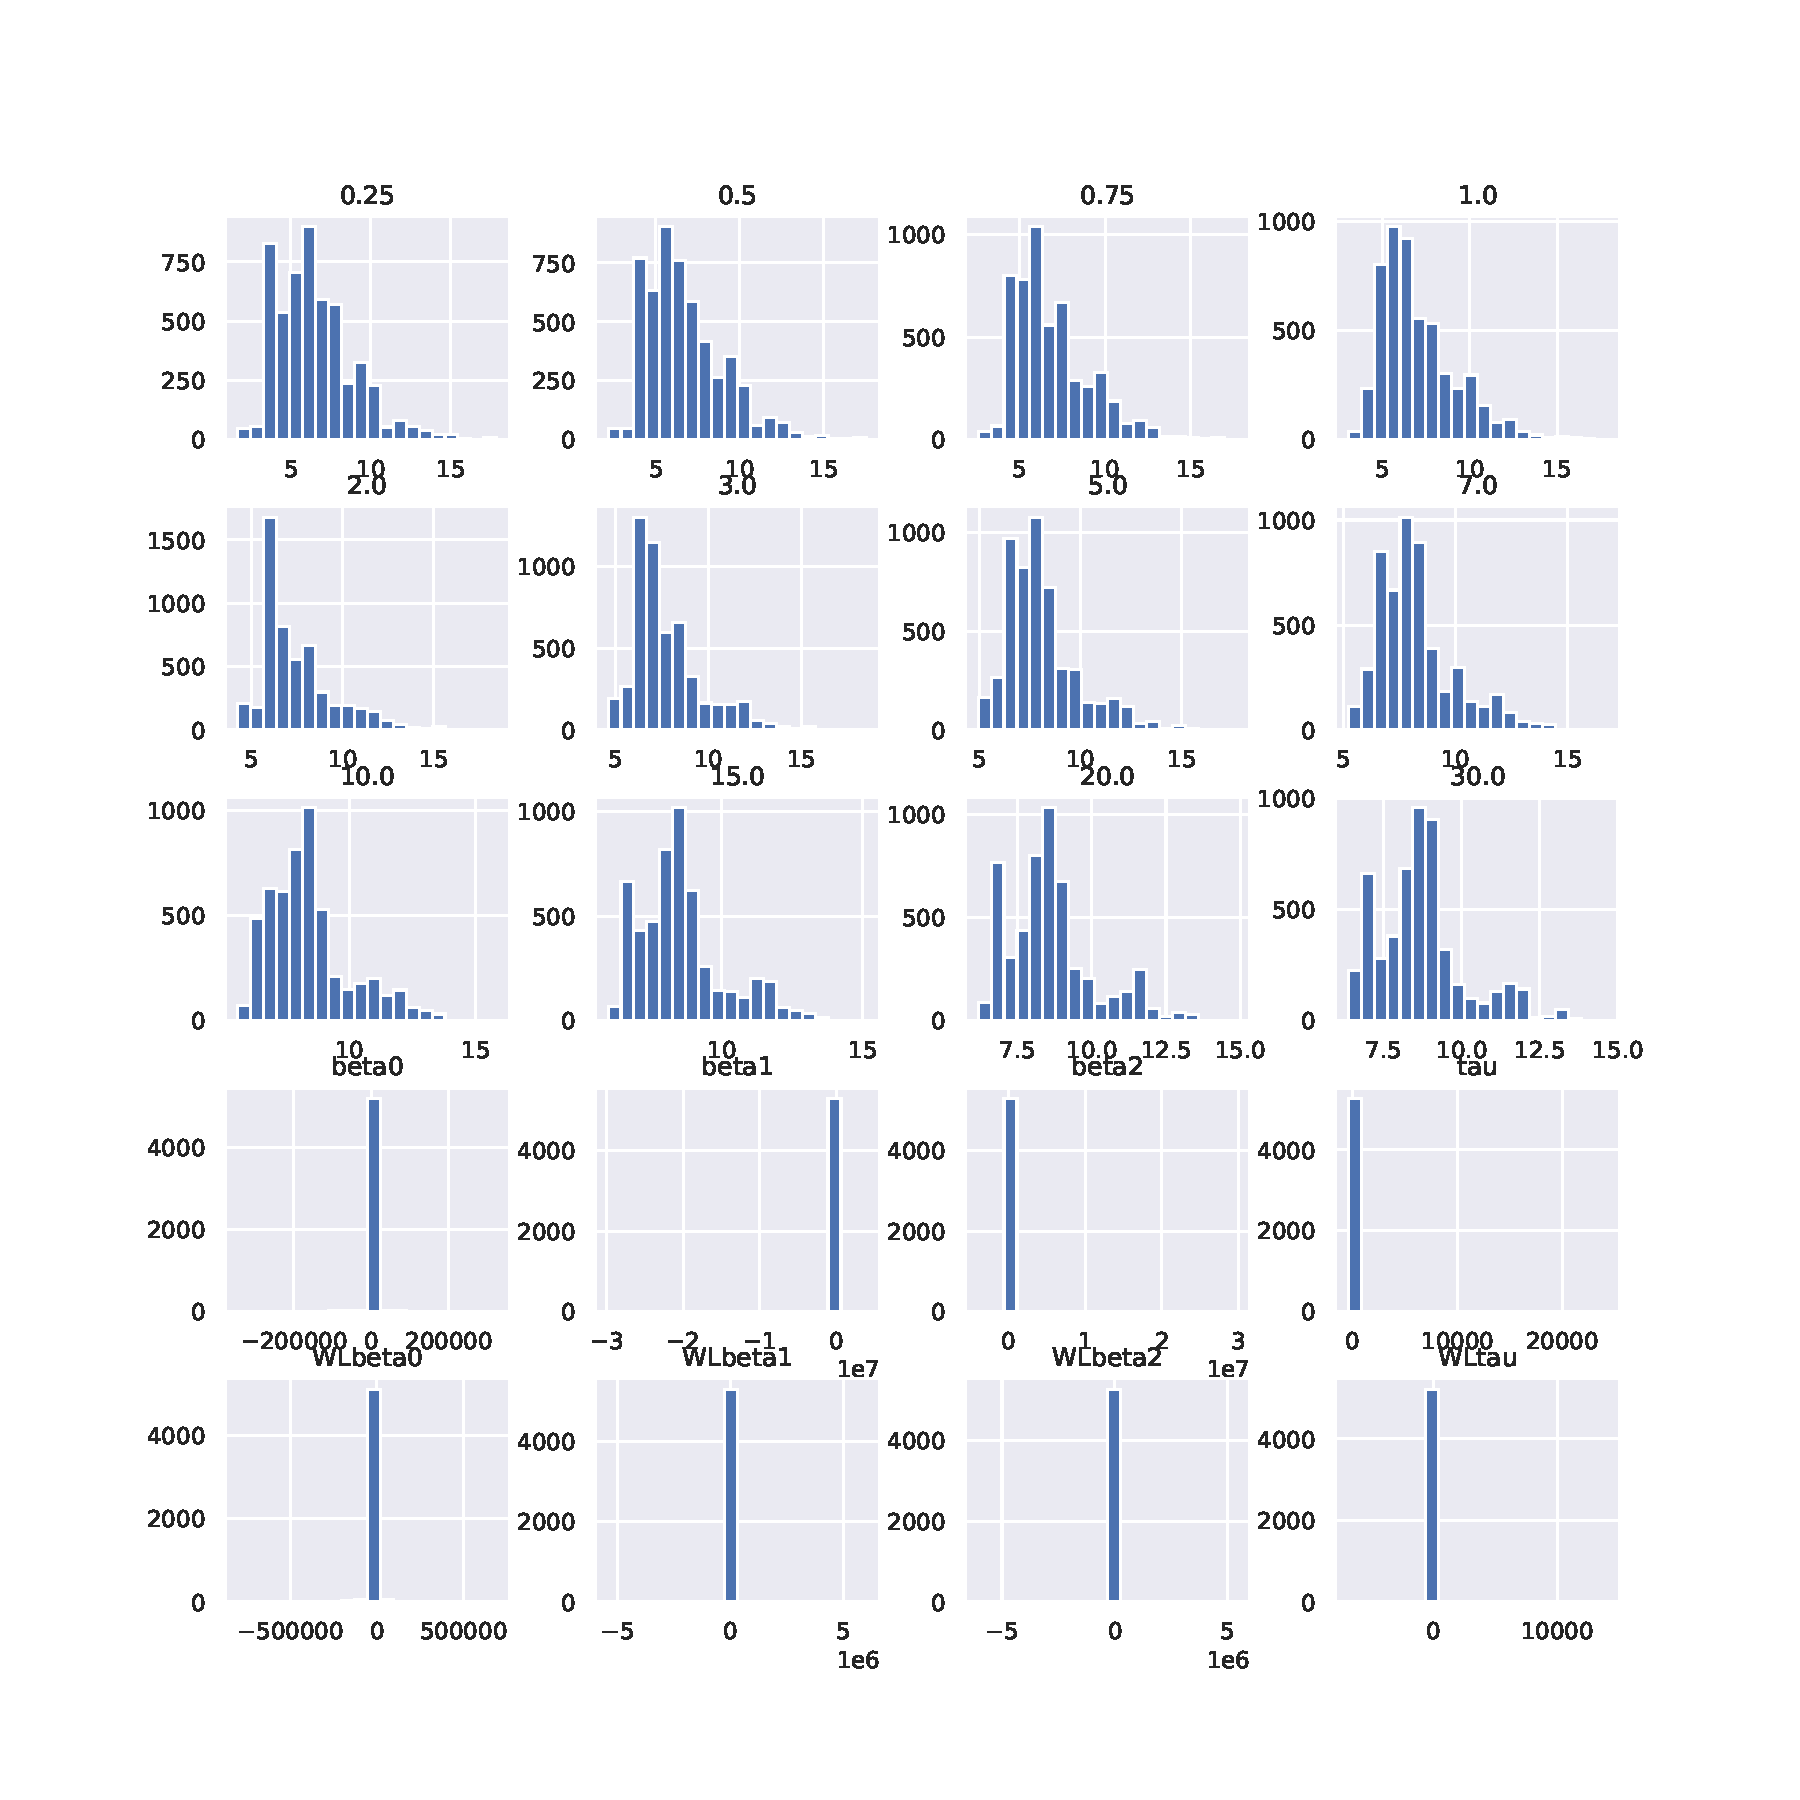
\includegraphics[width=\linewidth]{FactorHist.pdf}
                \caption{Nelson-Siegel factor distribution (with outliers)}
                \label{fig:NSHistOutliers}
            \end{figure}

            \begin{figure}
                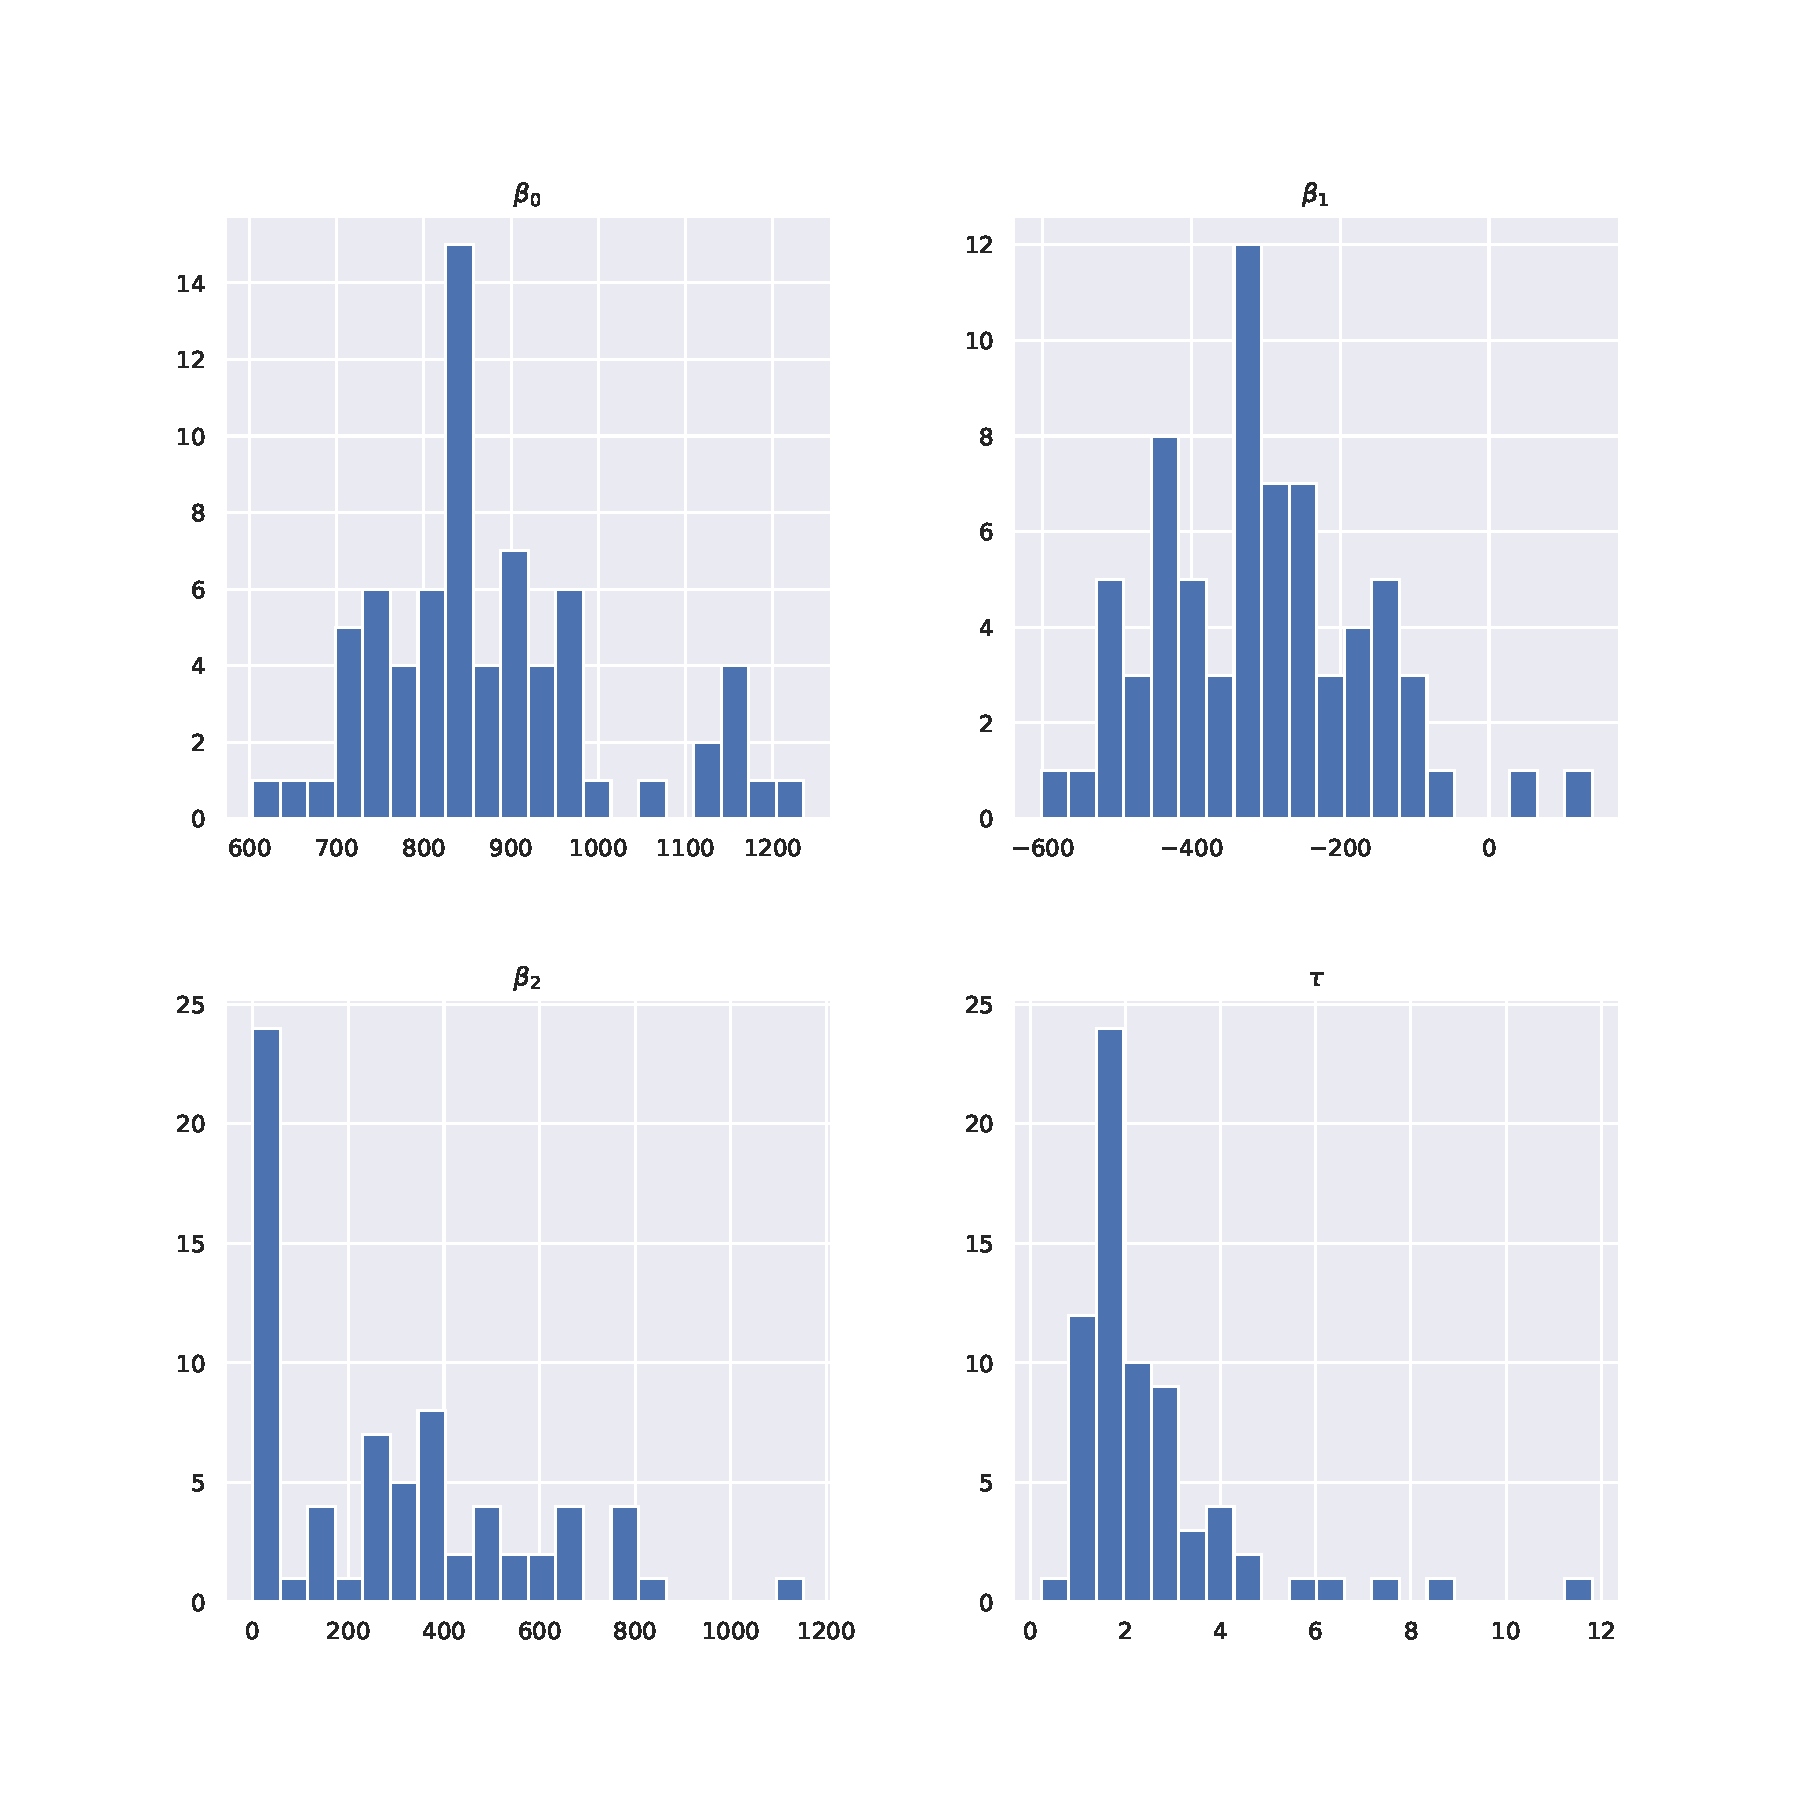
\includegraphics[width=\linewidth]{factorsAfterDrop.pdf}
                \caption{Nelson-Siegel factor distribution (without outliers)}
                \label{fig:NSHistDropped}
            \end{figure}

        \subsubsection{Forecasting results}
            To calibrate the suggested model we followed the steps described below:
            \begin{enumerate}
                \item Using the non-linear least squares method, we estimated the parameters of the static Nelson-Siegel 
                for each day of the sample period.
                \item Given a set of estimated factors, we estimated the parameters of the chosen model using the standard 
                OLS method. The models we used for the factor forecasting:
                    \begin{itemize}
                        \item auto-ARIMA,
                        \item VAR(1),
                        \item Random Walk as a baseline.
                    \end{itemize}
            \end{enumerate}

            After the non-linear least squares optimization, we obtained the factor dynamics found in Figure \ref{fig:factordynamics}.
            \begin{figure}
                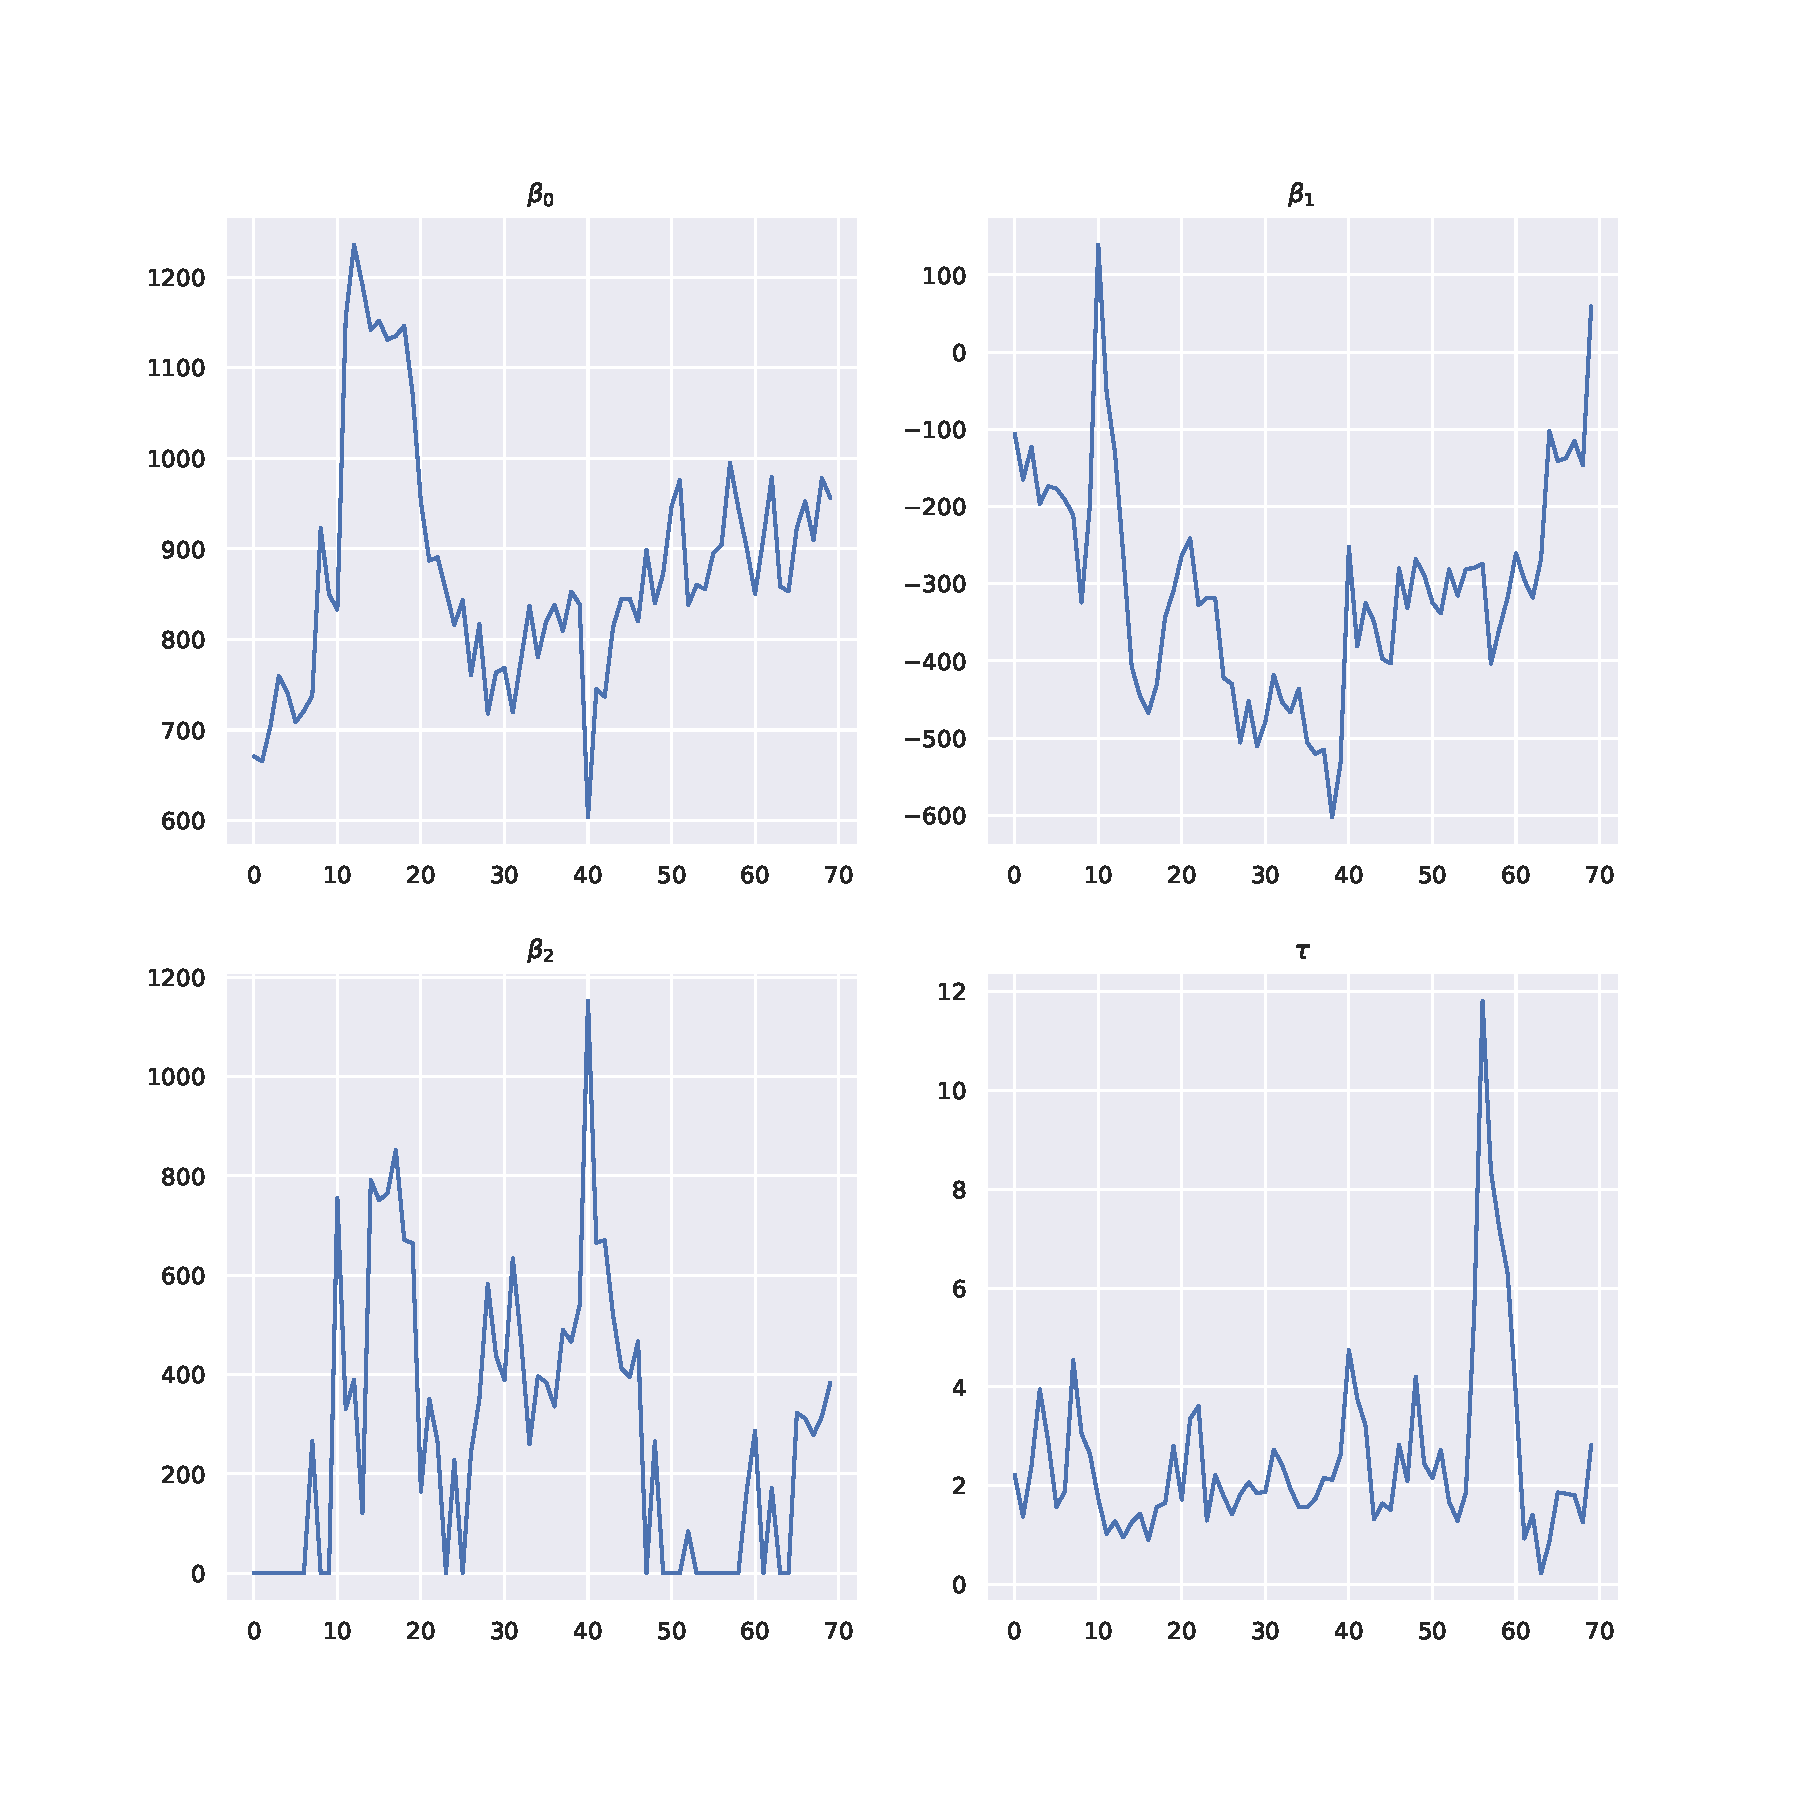
\includegraphics[width=\linewidth]{factors.pdf}
                \caption{Nelson-Siegel factor dynamics}
                \label{fig:factordynamics}
            \end{figure}

            It is possible to use the standard OLS method to estimate the parameters of the DNS model since there is 
            weak stationarity of the factor increments. 
            \subimport{results/NScoefsStationary}{diffNScoefsStationary}
            \subimport{results/NScoefsStationary}{NScoefsStationary}

            It turns out that the best forecast of the NS factors is the constant forecast. The results of the model calibration on a train dataset are presented 
            in Table \ref{tab:DNSresults}\footnote{Auto-ARIMA is not significantly better then RW. 
            All the other differences are significant at 1\% confidence level. We used Diebold-Mariano test. }.
            \begin{table}[htbp]
                \centering
                
\begin{comment}
     Здесь везде autoARIMA имеет порядок (0,0,0), кроме b2, там (1,0,0). Те в нашей фильтрации коэыыициенты модели - мартингалы.
\end{comment}

\begin{tabular}{|c | c c c|} 
    \hline
    Coefficient & autoARIMA & VAR(1) & RW \\ [0.5ex] 
    \hline
    $\beta_0$ & $53.78356$ & $131.1459$ & $66.3105$ \\ 
    \hline
    $\beta_1$ & $63.31042$ & $143.9235$ & $66.25878$ \\
    \hline
    $\beta_2$ & $133.9688$ & $388.3436$ & $177.1525$ \\
    \hline
    $\tau$ & $1.083687$ & $2.569167$ & $1.328986$ \\
    \hline
\end{tabular}
                \caption{Parameters of the DNS model for 3 different forecasting models.}
                \label{tab:DNSresults}
            \end{table}
